\documentclass[11pt]{article}
\usepackage[sort]{natbib}
\usepackage{bm,amsmath,bbm,amsfonts,nicefrac,latexsym,amsmath,amsfonts,amsbsy,amscd,amsxtra,amsgen,amsopn,bbm,amsthm,amssymb,graphicx}
\usepackage{fancyhdr}
\usepackage{wrapfig}
\usepackage{lscape}
\usepackage{rotating}
\usepackage[margin=0.8in]{geometry}
\bibliographystyle{plainnat}

\title{Thesis Outline}
\author{Ewan Pinnington}

\newtheorem{theorem}{Theorem}[section]
\newtheorem*{defn}{Definition}


\begin{document}

\maketitle

\section{Introduction}
\begin{itemize}
\item Why is understanding the carbon balance of forests important?
\item Terrestrial ecosystems and oceans are responsible for removing around half of all human emitted carbon-dioxide from the atmosphere and therefore greatly reduce the effect of anthropogenic induced climate change. Terrestrial ecosystem carbon uptake is the least understood process in the global carbon cycle. It is vital that we improve understanding in order to better constrain predictions of future carbon budgets (IPCC report).
\item Thesis aims and outline.
\end{itemize}


\section{Literature Review and Background}
\begin{itemize}
\item Variational data assimilation.
\item Representation of background and observation error and error correlations in data assimilation.
\item Ecosystem models.
\item DALEC2 and the processes it models.
\item Information Content (IC) measures.
\item Net Ecosystem Exchange (NEE) measurements, error and footprint model.
\end{itemize}


\section{Methods}
\begin{itemize}
\item Automatic differentiation for DALEC2 tangent linear model in Python (AlgoPy package).
\item Outline of Leaf Area Index (LAI) measurement campaign (ceptometer, hemispherical photographs and litter traps) and other work at Forest Research.
\end{itemize}


\section{4D-Var and improving the representation of background and observational error covariance matrices in carbon balance models}
\begin{itemize}
\item Work from the attached paper draft.
\item Implementation of DALEC2 in a 4D-Var scheme for parameter and state estimation.
\item Investigation into effect of including parameter-state error correlations in the background error covariance matrix, B, and correlations between observation errors in time in the observation error covariance matrix, R.
\item Results: Including parameter-state error correlations in B can significantly improve data assimilation forecast results. Including serial correlations between NEE observation errors in R also improves the assimilation forecast and we expect this to have a greater impact when assimilating more than one data stream.
\item Future work: Use Deroziers method to improve our estimates of both B and R. This will involve changing the Deroziers diagnostic so that it is applicable to a time window of observations in 4D-Var. Investigate the effect on our results from the data assimilation experiments. Using twin experiments with known error covariances to validate method.
\end{itemize}


\section{Information content in carbon balance observations with DALEC2}
\begin{itemize}
\item Introduce explicit expressions for information content for observations relating to DALEC2 at a single time.
\item Measures: Shannon information content, degrees of freedom for signal, influence matrix and adjoint sensitivity.
\item Consider IC in the context of a set of twin experiments using DALEC2.
\item Apply results to actual data acquired from Alice Holt.
\item Results: temporal information content in observations. What set of observations is best?
\item Investigate effect of data drop out, miss-specification of errors (twin experiments), quantity and time of sampling.
\item Investigate information content in NEE and Total Respiration (RT) observations when observations are treated as half hourly, averaged twice daily or averaged daily by using a variable time step in DALEC2.   
\end{itemize}


\section{Effect of disturbance on the Alice Holt research forest}
\begin{itemize}
\item Split NEE data into multiple data sets using flux tower footprint model, then parameterise DALEC2 for each data set. Compare the differences between the parameterisations with particular focus on the thinned/unthinned halves of the forest.
\item Compare the model parameters for LAI to observations taken in a planned field work campaign. From the field work is there a distinct difference between thinned/unthinned sides of the forest?
\item Implement a better phenology model in DALEC2 in order to improve our LAI estimates and possibly capture litter fall more accurately.
\item Inclusion of understory hazel in DALEC2, does this improve our estimates? Comparison with Eric Casella's version of SPA, parameterised for Alice Holt, which includes understory.
\end{itemize}


\section{Conclusion}
\begin{itemize}
\item Summary and future work.
\end{itemize}

\begin{sidewaysfigure}[ht]
    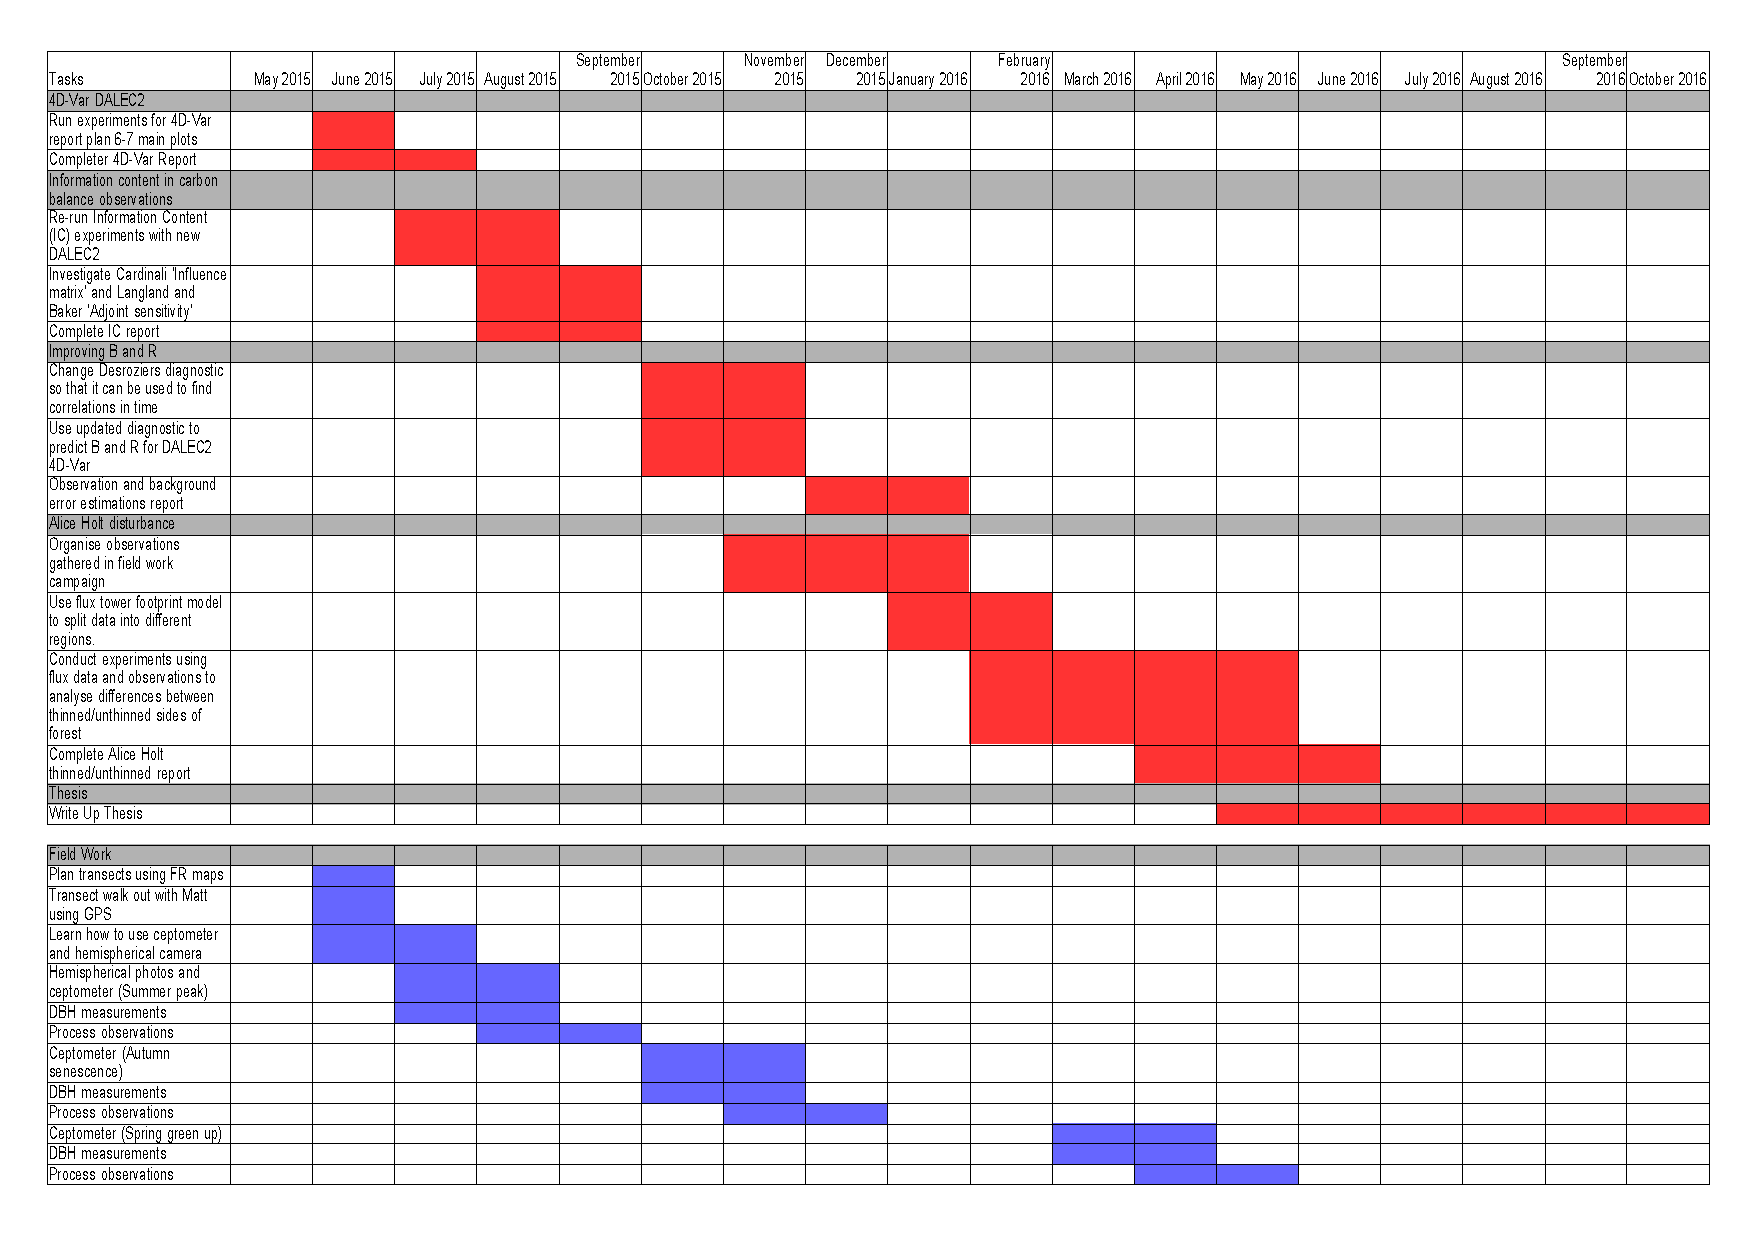
\includegraphics[width=1.\textwidth]{gantt.pdf}
    \caption{Gantt chart from monitoring committee 4.}
    \label{fig:PropProf}
\end{sidewaysfigure}

\begin{sidewaysfigure}[ht]
    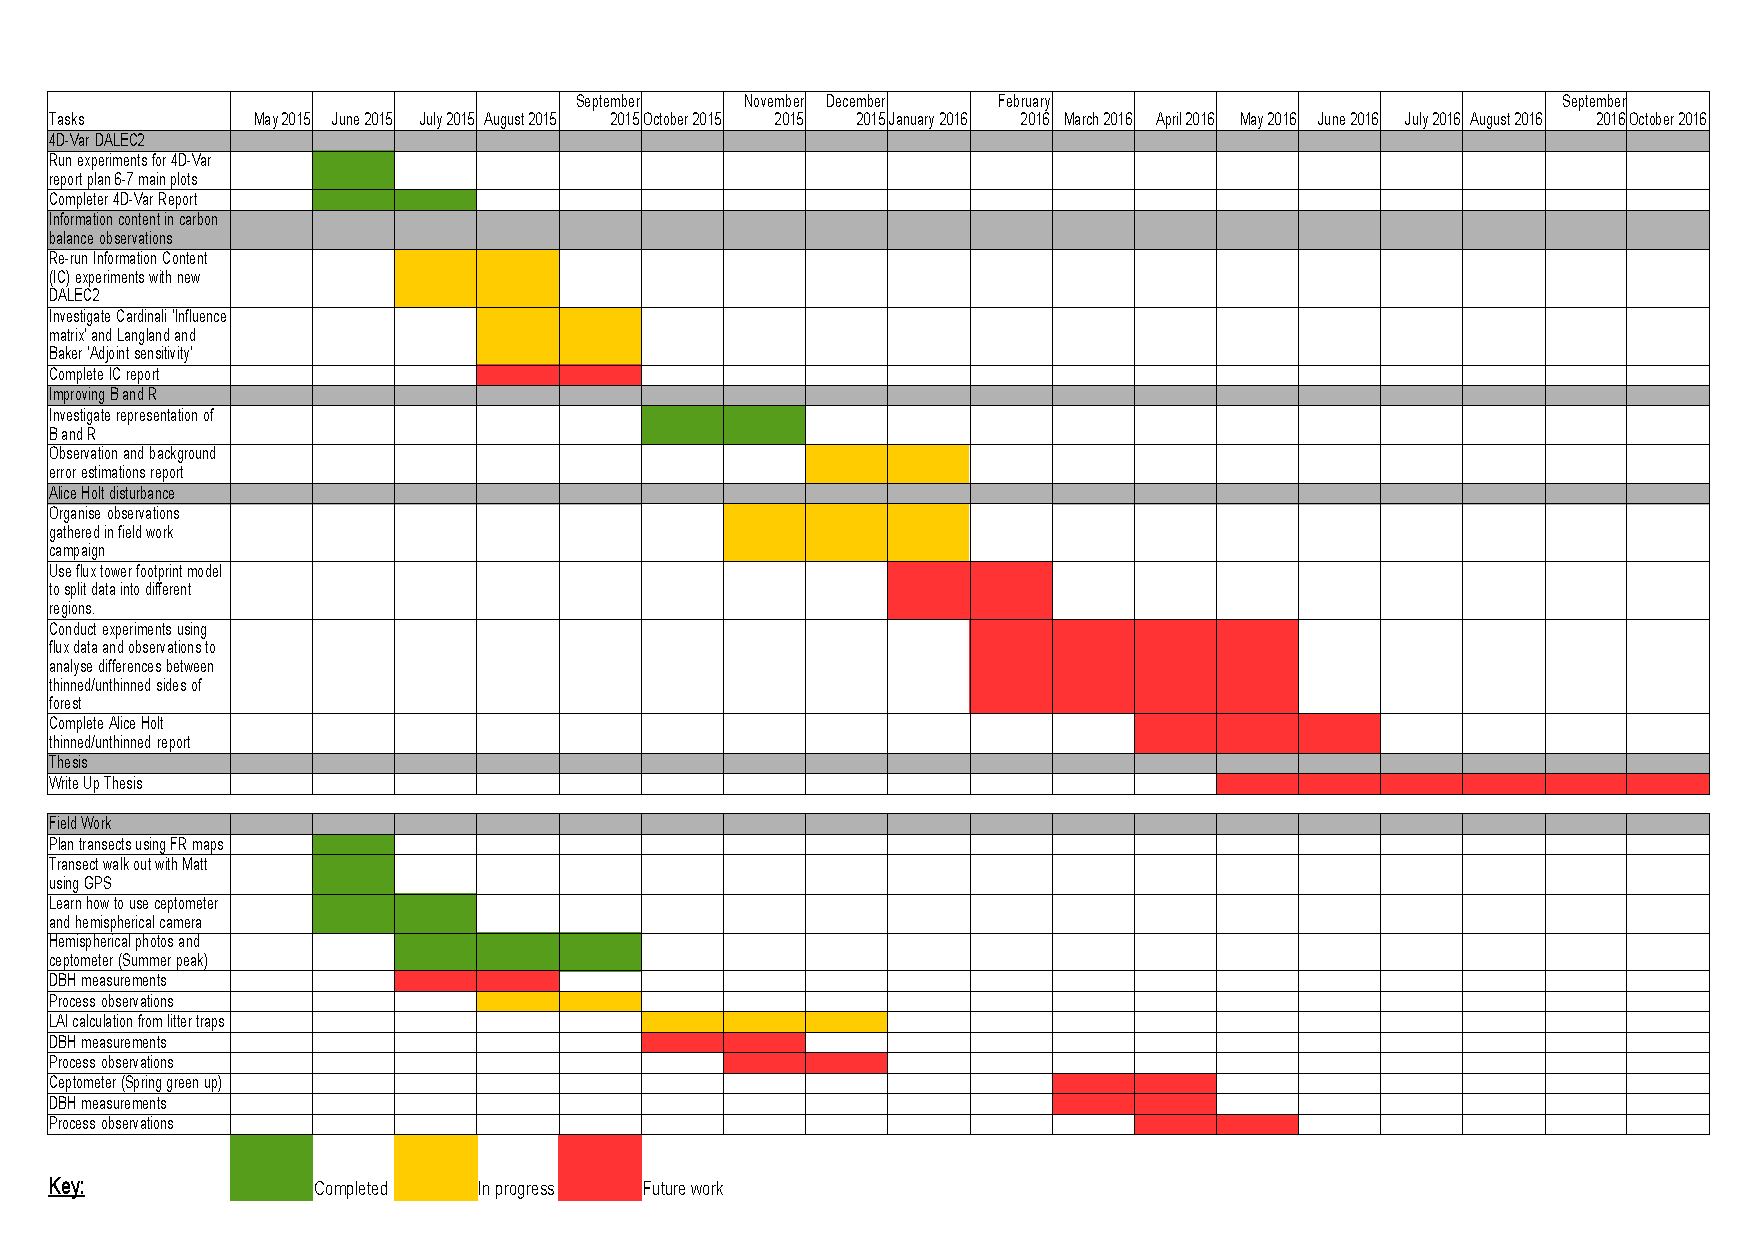
\includegraphics[width=1.\textwidth]{gantt_nov15.pdf}
    \caption{Updated Gantt chart from monitoring committee 5.}
    \label{fig:PropProf}
\end{sidewaysfigure}

\end{document}